\chapter{Playlists analysis}

Now we will move our focus from lyrics to playlists. Indeed, we will now demonstrate how we extended our work on single songs to whole playlists.

\section{Playlist classification}

Once we have a model to classify song emotions, our next step it trying to classify playlists emotion which could be a really useful information for a Recommender System which want to perform playlist continuation.

For the emotion classification task we decided to use three artificial neural networks, with the same architecture, but trained with three different datasets: MoodyLyrics, MoodyLyrics4Q and the merged dataset. Figure \ref{fig:annacc} shows the different accuracies reached with each dataset. 

\begin{figure}[H]
\centering
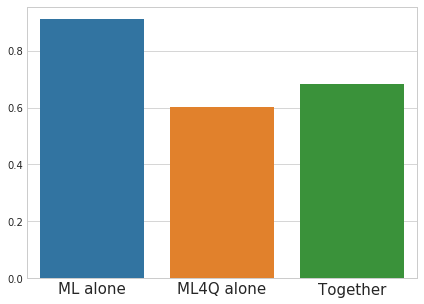
\includegraphics[width=0.7\textwidth]{./chapters/chapter5/images/ANN_accuracies.png}
\caption{5-fold ANN accuracies for each model}
\label{fig:annacc}
\end{figure}

The method we chose to classify a playlist is the following: given a \texttt{song emotion array} = [ sad\%, angry\%, happy\%, relaxed\% ] where the sum of the emotion percentage for each song is equal to one, the playlist emotion is the emotion with the maximum percentage column sum over the rows. We found this approach very flexible, indeed, normalizing by the number of songs inside a playlist we obtain a probability of the emotion for that playlist. This would add 4 additional features which could be used by a Recommendation System.

However our main issue has been the absence of a labeled dataset through which compute an accuracy score of our classification method. In order to overcome this problem a perfectly balanced silver standard dataset has been generated considering 40 playlist inside Spotify RecSys\cite{recsys} dataset with four really expressive titles: \textit{rage} for angry playlists, \textit{crying} for sad, \textit{party!} for happy and \textit{sleeping} for relaxed playlists. \par

The first step to classify the emotion for each song has been downloading the lyrics, but, unfortunately, we noticed that we could not download the entire number of song lyrics for every playlist. Figure \ref{fig:rsongs} shows, for each playlist, the number of songs for which we could download the lyrics, while figure \ref{fig:psongs} shows the percentage of available songs for each playlist. 

\begin{figure}[H]
\centering
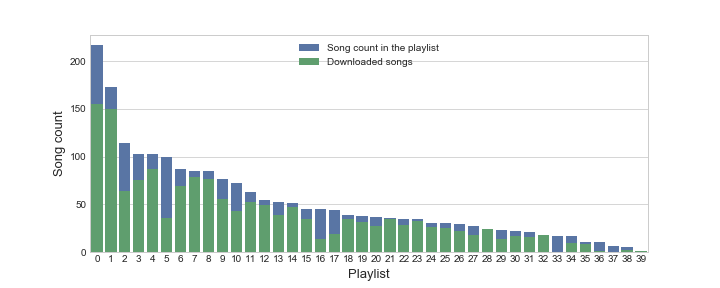
\includegraphics[width=1\textwidth]{./chapters/chapter5/images/silver_standard_available_songs.png}
\caption{Real number of available songs for playlist}
\label{fig:rsongs}
\end{figure}

\begin{figure}[H]
\centering
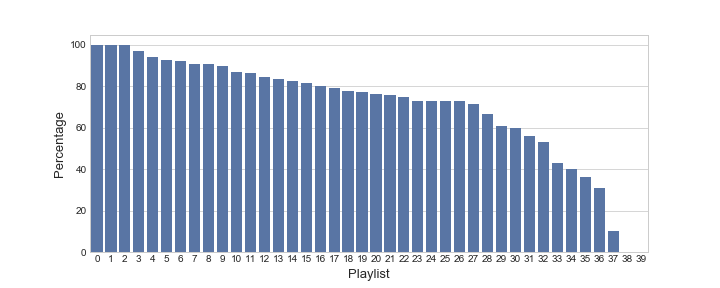
\includegraphics[width=1\textwidth]{./chapters/chapter5/images/silver_standard_percentage_available_songs.png}
\caption{Percentage of available songs for playlist}
\label{fig:psongs}
\end{figure}

Unfortunately two \textit{relaxed} playlist totally disappeared, unbalancing our silver standard.

We then featurized each song using the features described earlier in this report and classified them using the three artificial neural networks (one trained with MoodyLyrics, one with MoodyLyrics4Q and one with the merged datasets) we previously built.

\subsection{Robust Playlist Classification}

As we already said, playlist classification was done by averaging the emotion vectors which are given as output of the lyrics classification process. However, in order to make the classifications more robust, we tried to remove outliers from our predictions.

Basically, for each playlist, we built a matrix of dimension $N$x$4$, where $N$ is the number of songs in the playlist and $4$ is the number of target emotions (happy, sad, angry and relaxed). In this matrix, each row corresponds to the probabilistic assignment of emotions to each of song of the playlist. In order to remove outliers we considered a column (an emotion) at the time and we followed those steps:
\begin{enumerate}
\item compute the third (q3) and the first quartile (q1)
\item compute the interquartile range (IQR) defined as the difference between the third and the first quartile
\item define an upper bound value as $upper = q3 + (IQR * 1.5)$
\item define a lower bound value as $lower = q1 - (IQR * 1.5)$
\item eliminate from the column all those values outside the range $[lower, upper]$
\item average the remaining values to compute the label score for the emotion corresponding to the current column of the matrix
\end{enumerate}

After having repeated the above process for all the $4$ columns of our $N$x$4$ matrix, we obtain a vector of $4$ real values, respectively representing the playlist score for each of our target emotion.

\subsection{Playlist Classification with a subset of the songs}

In order to improve our computational speed we came up with the idea that probably a playlist's emotion is clearly expressed in just a subset of its songs, making it useless to compute emotion classification of each of its song. For this purpose, we tried to consider just a small sample of the total songs at the time, incrementally increasing our sample size.

We did this operation both using our simple, average based, classification scheme and the other, more robust, and outlier sensitive approach.

Figures \ref{fig:subset-absolute} and \ref{fig:subset-percentage} shows the accuracy results obtained while using the simple average classification approach, while figures \ref{fig:subset-absolute-robust} and \ref{fig:subset-percentage-robust} shows the results obtained while using the robust classification approach.

\begin{figure}[H]
\centering
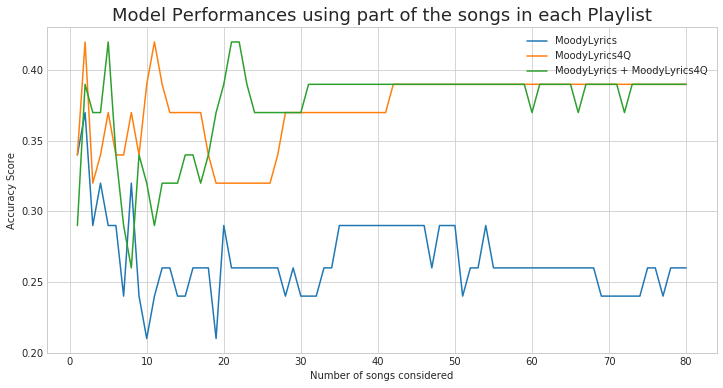
\includegraphics[width=0.9\textwidth]{./chapters/chapter5/images/subset-absolute}
\caption{Classification accuracy on playlists obtained while considering just a certain amount of songs}
\label{fig:subset-absolute}
\end{figure}

\begin{figure}[H]
\centering
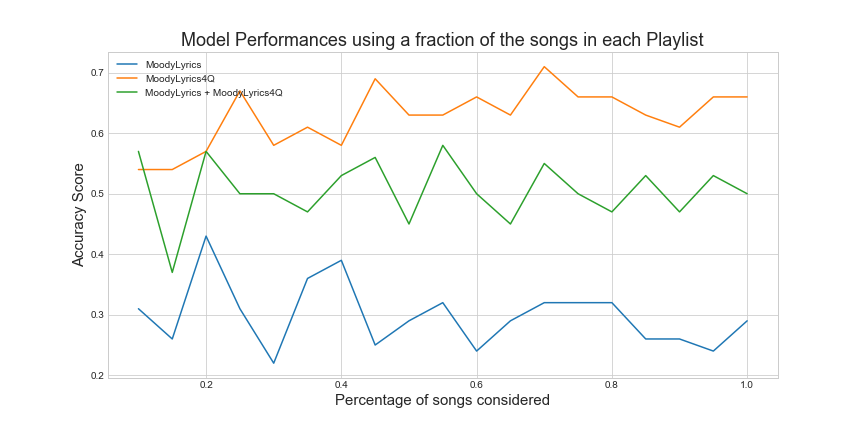
\includegraphics[width=0.9\textwidth]{./chapters/chapter5/images/subset-percentage}
\caption{Classification accuracy on playlists obtained while considering just a percentage sample of the total number of songs}
\label{fig:subset-percentage}
\end{figure}

\begin{figure}[H]
\centering
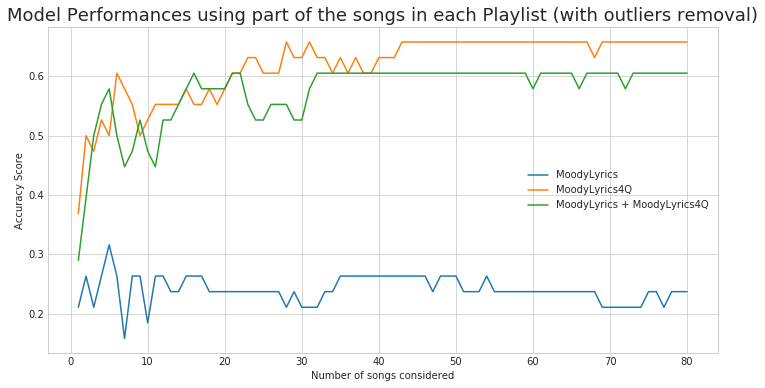
\includegraphics[width=0.9\textwidth]{./chapters/chapter5/images/subset-absolute-robust}
\caption{Classification accuracy on playlists obtained using robust classification while considering just a certain amount of songs}
\label{fig:subset-absolute-robust}
\end{figure}

\begin{figure}[H]
\centering
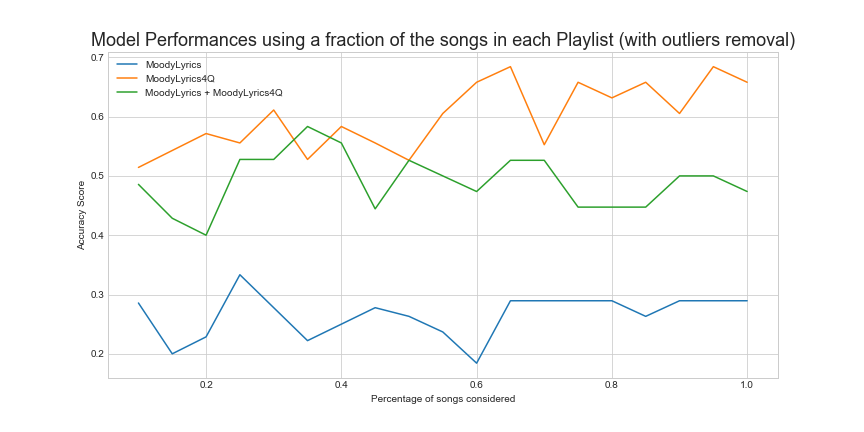
\includegraphics[width=0.9\textwidth]{./chapters/chapter5/images/subset-percentage-robust}
\caption{Classification accuracy on playlists obtained while using robust classification considering just a percentage sample of the total number of songs}
\label{fig:subset-percentage-robust}
\end{figure}

As we can see from those figures, in order to converge to a stable classification accuracy value, the algorithm always needs a huge number of songs. Therefore we believed that this experiment told us that, the best way to classify our playlists is still to consider all of the songs contained in them.

\subsection{Results}
Table \ref{tab:comparison2} shows the different accuracies reached classifying the playlist emotions using the method previously explained. 

\begin{table}[H]
\centering
\begin{tabular}{ |p{3cm}||p{1.5cm}|p{1.5cm}| }
 \hline
 \multicolumn{3}{|c|}{Playlist Classification Accuracy} \\
 \hline
Dataset & With outliers & Without outliers\\
 \hline
MoodyLyrics & 29\% & 29\%\\
MoodyLyrics4Q  & 66\%    &66\%\\
Both together &   50\%  & 47\%\\
\hline
\end{tabular}
\caption{Playlist classification accuracies comparison} \label{tab:comparison2}
\end{table}

\section{Emotion patterns in playlists}


\begin{figure}[H]
  \centering
  \begin{subfigure}[b]{0.49\linewidth}
    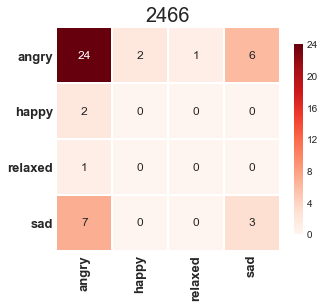
\includegraphics[width=\linewidth]{./chapters/chapter5/images/2466.png}
    \caption{Playlist PID 2466}
  \end{subfigure}
  \begin{subfigure}[b]{0.49\linewidth}
   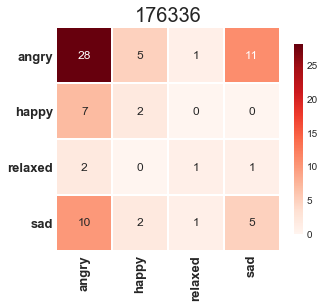
\includegraphics[width=\linewidth]{./chapters/chapter5/images/176336.png}
    \caption{Playlist PID 176336}
  \end{subfigure}
  \caption{Rage playlists pattern}
  \label{fig:ann}
\end{figure}

\begin{figure}[H]
  \centering
  \begin{subfigure}[b]{0.49\linewidth}
    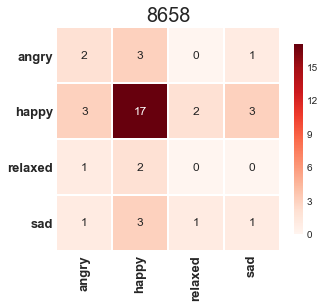
\includegraphics[width=\linewidth]{./chapters/chapter5/images/8658.png}
    \caption{Playlist PID 8658}
  \end{subfigure}
  \begin{subfigure}[b]{0.49\linewidth}
   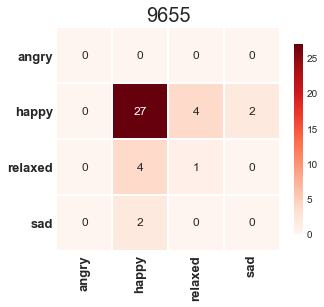
\includegraphics[width=\linewidth]{./chapters/chapter5/images/9655.png}
    \caption{Playlist PID 9655}
  \end{subfigure}
  \caption{Happy playlists pattern}
  \label{fig:ann}
\end{figure}

\begin{figure}[H]
  \centering
  \begin{subfigure}[b]{0.49\linewidth}
    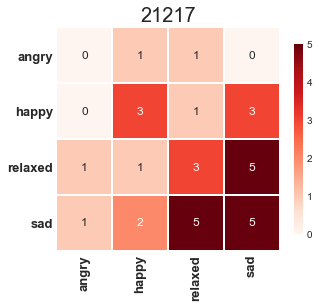
\includegraphics[width=\linewidth]{./chapters/chapter5/images/21217.png}
    \caption{Playlist PID 21217}
  \end{subfigure}
  \begin{subfigure}[b]{0.49\linewidth}
   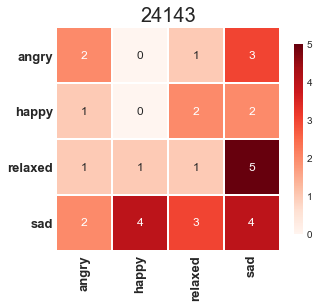
\includegraphics[width=\linewidth]{./chapters/chapter5/images/24143.png}
    \caption{Playlist PID 24143}
  \end{subfigure}
  \caption{Relaxed playlists pattern}
  \label{fig:ann}
\end{figure}

\begin{figure}[H]
  \centering
  \begin{subfigure}[b]{0.49\linewidth}
    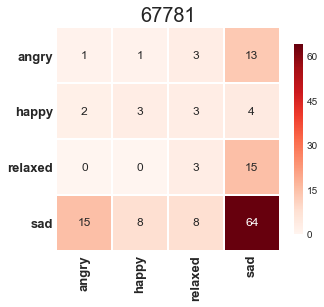
\includegraphics[width=\linewidth]{./chapters/chapter5/images/67781.png}
    \caption{Playlist PID 67781}
  \end{subfigure}
  \begin{subfigure}[b]{0.49\linewidth}
   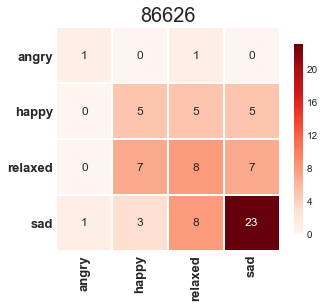
\includegraphics[width=\linewidth]{./chapters/chapter5/images/86626.png}
    \caption{Playlist PID 86626}
  \end{subfigure}
  \caption{Sad playlists pattern}
  \label{fig:ann}
\end{figure}











